\label{Grundlagen der IT-Sicherheit}
%\begin{section}{Grundlagen der IT-Sicherheit}
 In diesem Kapitel werden allgemeine Begriffe wie zum Beispiel die Grundbegriffe der
 Sicherheit, diverse Sicherheitsziele aus dem Grundschutzkatalog sowie Schutzbedarf 
 Bedrohungsanalysen behandelt. 
 \\
 Weiters wird eine klare Grenze zwischen Sicherheit und IT-Sicherheit gezogen. 
 Abschließend wird auf das Teilgebiet der VoIP-Sicherheit eingegangen.
 \\
%\end{section}

 \label{Sicherheitsziele}
 \begin{section}{Sicherheitsziele}
  Das deutsche Bundesamt für Sicherheit in der Informationstechnik (BSI) beschreibt 
  folgende Sicherheitsziele (security objectives) in einem Sicherheitskatalog: 
  \cite{BSIBedarf}
  \begin{itemize}
   \item Verfügbarkeit (availability)
   \item Integrität (integrity)
   \item Vertraulichkeit (privacy, confidentialty)
  \end{itemize}
  \pagebreak

   \DIFdelbegin %DIFDELCMD < \begin{subsection}{Verfügbarkeit}
%DIFDELCMD <     %%%
\DIFdel{Verfügbarkeit (availability) meint die Eigenschaft eines Systems, innerhalb eines 
    bestimmten Zeitraums mit einer bestimmten Wahrscheinlichkeit die vom eingesetzten 
    System erwarteten Anforderungen zu erfüllen. Die Verfügbarkeit zählt zu den 
    Qualitätsmerkmalen einer IT-Landschaft.
    }%DIFDELCMD < \\
%DIFDELCMD <    \end{subsection}
%DIFDELCMD < 

%DIFDELCMD <    %%%
\DIFdelend \label{Integrität}
   \begin{subsection}{Integrität}
    Unter der Integrität (integrity) \DIFaddbegin \cite{BSIa} \DIFaddend von Informationen versteht man die Vollständigkeit und 
    Korrektheit (Unversehrtheit) der übertragenen Daten auf Sender- und auch Empfängerseite \DIFaddbegin \cite{BSIInfosi}\DIFaddend . 
    Dabei wird davon ausgegangen, dass keine Manipulation der Daten auf dem Transportweg 
    durchgeführt wurden und somit unveränderte Daten verschickt wurden. Um diese 
    Datenintegrität an beiden Kommunikationsenden zu kontrollieren, kann man verschiedene 
    Kontrollmethoden verwenden: \ac{Z.B.} Hash-Verfahren, message authentification codes 
    oder digitale Signaturen \DIFaddbegin \cite{BSIBegriffe1}\DIFaddend . Um diesen Mechanismus durchführen zu können, sind die Inhalte 
    der Daten mit den Kontrollmethoden direkt verknüpft. 
    Durch unzureichende Integritätsprüfung können fehlerhafte Datensätze entstehen: Z.B. 
    Fehlerhafte Produktionen, Falsche Warenlieferungen oder Verbuchungsfehler. 
    In den letzten Jahren wird dem Verlust an Authentizität als Teil der Datenintegrität 
    verstärktes Augenmerk gewidment. 
    Im schlimmsten Fall wirken sich Fehler auf Zahlungen und Identitäten aus, welche an 
    nicht berechtigte Personen ausgestellt werden. So kann es beispielsweise zu 
    Identitätsdiebstahl kommen.    
    \DIFdelbegin %DIFDELCMD < \cite{BSIInfosi} \cite{BSIa} \cite{BSIBegriffe1}
%DIFDELCMD <     %%%
\DIFdelend \\
   \end{subsection}

   \DIFaddbegin \label{Verfügbarkeit}
   \begin{subsection}{Verfügbarkeit}
    \DIFadd{Verfügbarkeit (availability) meint die Eigenschaft eines Systems, innerhalb eines 
    bestimmten Zeitraums mit einer bestimmten Wahrscheinlichkeit die vom eingesetzten 
    System erwarteten Anforderungen zu erfüllen. Die Verfügbarkeit zählt zu den 
    Qualitätsmerkmalen einer IT-Landschaft.
    }\\
   \end{subsection}

   \DIFaddend \label{Vertraulichkeit}
   \begin{subsection}{Vertraulichkeit}
    Um eine sichere und effektive Datenübertragung und Verarbeitung zu gewährleisten, muss 
    eine hohe Vertraulichkeit (confidentiality) erreicht werden und erhalten bleiben. 
    Allgemein lässt sich die Vertraulichkeit als Gewährleistung beschreiben, bei welcher die 
    zu verarbeitenden Daten nur an jene Personen zugestellt und verfügbar gemacht werden, die 
    auch die nötigen Berechtigungen besitzen. Auf der anderen Seite werden Personen mit 
    keinerlei Berechtigung von den Daten separiert.
    \\
    \end{subsection}
    \DIFaddbegin \pagebreak
\DIFaddend 

   \DIFdelbegin %DIFDELCMD < \label{Zuverlässigkeit}
%DIFDELCMD <     \begin{subsection}{Zuverlässigkeit}
%DIFDELCMD <      %%%
\DIFdelend \DIFaddbegin \label{Ergänzung: Zuverlässigkeit}
    %DIF > \begin{subsection}{Zuverlässigkeit}
   \DIFadd{\textbf{Ergänzung: Zuverlässigkeit} }\\ \\
     \DIFaddend Microsoft definiert sechs Merkmale, welche auf einem System angewandt werden sollen. 
     Diese Qualitätsmerkmale bestehen im Wesentlichen aus den oben genannten Komponenten 
     Verfügbarkeit und Integrität.
     %DIF > \cite{Micro05}
     \begin{enumerate} 
      \item ausfallsicher \\
       Das System kann dem Benutzer auch dann Dienste anbieten, wenn eine interne oder 
       externe Unterbrechung stattfindet. (Verfügbarkeit)
      \item wiederherstellbar \\
       Das System kann nach einer benutzerbedingten oder systembedingten Unterbrechung 
       mittels Instrumentation oder Diagnose problemlos wieder ohne Datenverlust in seinen 
       ursprünglichen Zustand zurückgeführt werden. (Verfügbarkeit)
      \item kontrolliert \\
       Das System erfüllt im Bedarfsfall immer korrekt und rasch die Anforderungen an den 
       gewünschten Dienst. (Verfügbarkeit, Integrität)
      \item unterbrechungsfrei \\
       Erforderliche Änderungen und Aktualisierungen unterbrechen den Systembetrieb nicht. 
       (Verfügbarkeit)
      \item produktionsbereit \\
       Das System weist bereits bei der Auslieferung nur ein Minimum an Fehlern auf, 
       wodurch nur eine begrenzte Zahl an vorhersehbaren Aktualisierungen nötig ist. 
       (Verfügbarkeit)
      \item berechenbar \\
       Das System funktioniert wie erwartet bzw. wie vereinbart. Die Funktionalität von 
       früher bleibt weiter erhalten. (Verfügbarkeit, Integrität) \\      
     \DIFdelbegin %DIFDELCMD < \cite{Micro05}
%DIFDELCMD <      %%%
\DIFdelend \end{enumerate}
    \DIFdelbegin %DIFDELCMD < \end{subsection}
%DIFDELCMD <   %%%
\DIFdelend %DIF > \end{subsection}
    \DIFaddbegin \pagebreak
  \DIFaddend \end{section}

 \label{Schutzbedarf}
 \begin{section}{Schutzbedarf}
  Der Schutz von Daten und Informationsflüssen gehört für die Unternehmen und öffentlichen
  Einrichtungen von heute zu den heikelsten und wichtigsten Aufgaben. Ständig aktuelle 
  Daten sind ein unerlässliches Gut für Unternehmen und sollten ständig auf dem neuesten 
  Stand sein. Um diese Daten-Updates durchführen zu können, werden möglichst viele 
  Informationen auf Datenträgern persistent gespeichert. Dabei kann sichergestellt werden, 
  dass diese Daten keinem Risiko ausgesetzt sind sondern mittels spezieller Methodik 
  gesichert und verwahrt werden. Andererseits gibt es aber auch Daten, welche nicht oder 
  nur schwach gesichert werden. Dies kann im schlimmsten Fall zum Verlust von Daten und 
  erheblichen Geldbeträgen führen. Grundlegende Sicherheitsmaßnahmen sind mithilfe von 
  geringen Mitteln und Maßnahmen zu erreichen. \\
  \\
  Der Schutzbedarf "Hoch" bedeutet, dass für die Abdeckung dieser Schutzkategorien 
  spezielle Maßnahmen ergriffen werden müssen. 
  Das \ac{BSI} stellte eine Zusammenstellung aus IT-Grundschutz-Vorgehensweisen und IT-Grundschutzkatalogen
  an, welche die Voraussetzungen für den Einsatz in den unterschiedlichsten Umgebungen 
  darstellt. \\
  \\
  Der Trend zur Speicherung aller Arten von Daten gehört genauso zum alltäglichen Leben 
  wie der Computer selbst. Von Vorratsdatenspeicherung bis hin zu Onlinedatenspeicherung 
  vernetzt über den Globus betrifft das Thema fast jeden Menschen. Selbst der Staat setzt 
  bei Speicherung von Patientendaten und Steuerdaten auf Informationsvernetzung und - speicherung.   
  \DIFdelbegin %DIFDELCMD < \\
%DIFDELCMD <   \\
%DIFDELCMD <   %%%
\DIFdelend \DIFaddbegin \pagebreak

  \DIFaddend Um den teilweise öffentlichen Forderung an Konsistenz und Sicherheit nachkommen zu 
  können, muss der Sicherheitsgrad hoch und der Schutzbedarf gedeckt sein. 
  Schutzbedarf selbst ist nicht quantifizierbar - aber das \ac{BSI} teilt diesen in drei 
  Kategorien: \DIFaddbegin \cite{BSIBedarf} \DIFaddend \\
  \begin{enumerate} 
   \item Normal \\
    Die Schadensauswirkungen sind begrenzt und überschaubar.
   \item Hoch \\
    Die Schadensauswirkungen können beträchtlich sein.
   \item Sehr Hoch \\
    Die Schadensauswirkungen können ein existentiell bedrohliches bzw. katastrophales 
    Ausmaß erreichen. 
  \DIFdelbegin %DIFDELCMD < \cite{BSIBedarf}
%DIFDELCMD <   %%%
\DIFdelend \end{enumerate}
  \DIFdelbegin %DIFDELCMD < \pagebreak
%DIFDELCMD < %%%
\DIFdelend 

  Die Sicherheit von Daten und Systemen beschränkt sich heute nur auf technische 
  Gegebenheiten sondern umfasst auch die Sicherheit von organisatorischen und personellen 
  Umgebungsvariablen. Bei diesen ist es enorm wichtig, dass man behutsam und mit großer 
  Flexibilität ans Werk geht. Des Weiteren ist es wichtig, dass mit der richtige Umgang 
  mit sensiblen Daten und mit Betriebsvariablen sichergestellt wird. \\
  \\
  Für die heutigen Entwicklungsschritte in der Vernetzungstechnologie sind folgende 
  Faktoren prägend: \DIFaddbegin \cite{BSIa} \DIFaddend \\

  \begin{enumerate} 
   \item Vernetzung \\
    Das Phänomen der Vernetzung wurden in den letzten Jahren durch Internet, VoIP und 
    viele andere technische Errungenschaften verstärkt. Die rasante Entwicklung in den 
    letzten zwei Jahrzehnten hat gezeigt, dass heute nicht mehr isoliert und lokal 
    gebunden gearbeitet wird, sondern mit verschiedenen Rechner und Menschen rund um den 
    Globus kommuniziert wird. Die globale Vernetzung bietet viele verschiedene 
    Möglichkeiten für verteiltes Arbeiten. So können etwa verteilte Ressourcen, gemeinsam 
    genutzte Datenbestände und Cloudcomputing zum eigenen Vorteil genutzt werden. \\

   \item IT-Verarbeitung und Durchdringung \\
 	Im Alltag finden wir heute viele IT-Geräte, die uns das Leben leichter machen sollen.
 	Immer kleiner werdende Teile werden in den unterschiedlichsten Bereichen eingesetzt - vom Auto 
 	bis hin zur Küche. Der wohl aktuellste Lebensbereich ist jener der Mobiltelefonie.
 	Kaum jemand besitzt keine Mobiltelefon, welches im Laufe der letzten Jahre zu einem integralen 
 	Bestandteil der modernen Gesellschaft wurde.

   \item Schwindende Netzgrenzen \\
 	Vor wenigen Jahren war die Softwareentwicklung noch in geographisch lokalen Gebieten eingrenzbar.
 	Doch mittlerweile haben sich einige Bewegungen und Firmen formiert, die ihre Softwareentwicklung 
 	auf verschiedene Teams an verschiedenen Orten der Welt aufteilen.
 	Somit ergeben sich nicht gegebenenfalls nicht nur finanzielle sondern auch organisatorische 
 	Vorteile.  \\   
 	 	\DIFdelbegin %DIFDELCMD < \cite{BSIa} 	
%DIFDELCMD <  	%%%
\DIFdelend 

 	
   \end{enumerate}
 \end{section}

 \label{IT-Schutzkataloge}
 \begin{section}{IT-Schutzkataloge}
	Der Grundschutzkatalog des BSI ist ein Werk einer deutschen Institution, welches 
	internationales Ansehen genießt. Der gesamte Inhalt wird auch in englischer Sprachen 
	angeboten.
	BSI-Standards enthalten Empfehlungen des BSI zu Methoden, Prozessen und Verfahren sowie Vorgehensweisen 
	und Maßnahmen mit Bezug zur Informationssicherheit. 
	Das BSI greift dabei Themenbereiche auf, die von grundsätzlicher Bedeutung für die 
	Informationssicherheit in Behörden oder Unternehmen sind und für die sich national oder 
	international sinnvolle und zweckmäßige Herangehensweisen etabliert haben.
	Einerseits dienen BSI-Standards zur fachlichen Unterstützung von Anwendern der Informationstechnik. 
	Das erleichtert die sichere Nutzung von Informationstechnik, da auf bewährte Methoden, Prozesse 
	oder Verfahren zurückgegriffen werden kann.
  \cite{BSIITkat}  
  \DIFdelbegin %DIFDELCMD < 

%DIFDELCMD <   \pagebreak
%DIFDELCMD <   %%%
\DIFdelend %DIF > \pagebreak
  Auszug auf den Grundschutzstandards:
  \begin{enumerate}
	\item BSI-Standard 100-1 \DIFaddbegin \cite{BSIGSStd}\DIFaddend : \ac{ISMS} \\
		\DIFaddbegin \DIFadd{Der vorliegende BSI-Standard definiert allgemeine Anforderungen an ein ISMS.
	}\DIFaddend \item BSI-Standard 100-2 \DIFaddbegin \cite{BSIGSStd}\DIFaddend : IT-Grundschutz-Vorgehensweise \\
		\DIFaddbegin \DIFadd{Die IT-Grundschutz-Vorgehensweise beschreibt Schritt für Schritt, 
		wie ein Managementsystem für Informationssicherheit in der Praxis aufgebaut 
		und betrieben werden kann. Die Aufgaben des Sicherheitsmanagements und 
		der Aufbau von Organisationsstrukturen für Informationssicherheit sind dabei wichtige Themen.
	}\DIFaddend \item BSI-Standard 100-3 \DIFaddbegin \cite{BSIGSStd}\DIFaddend : Risikoanalyse auf der Basis von IT-Grundschutz \\
		\DIFaddbegin \DIFadd{Die IT-Grundschutz-Kataloge des BSI enthalten Standard-Sicherheitsmaßnahmen 
		aus den Bereichen Organisation, Personal, Infrastruktur und Technik, 
		die bei normalen Sicherheitsanforderungen in der Regel angemessen und 
		ausreichend zur Absicherung von typischen Geschäftsprozessen und Informationsverbünden sind.
	}\DIFaddend \item BSI-Standard 100-4 \DIFaddbegin \cite{BSIGSStd}\DIFaddend : Notfallmanagement \\
		\DIFaddbegin \DIFadd{Mit dem BSI-Standard 100-4 wird ein systematischer Weg aufgezeigt, 
		ein Notfallmanagement in einer Behörde oder einem Unternehmen aufzubauen, 
		um die Kontinuität des Geschäftsbetriebs sicherzustellen. Aufgaben eines Notfallmanagements sind daher, 
		die Ausfallsicherheit zu erhöhen und die Institution auf Notfälle und Krisen adäquat vorzubereiten, 
		damit die wichtigsten Geschäftsprozesse bei Ausfall schnell wieder aufgenommen werden können.
  }\DIFaddend \end{enumerate}
 \end{section}

 \label{Aufbau Grundschutzkataloge}
 \DIFdelbegin %DIFDELCMD < \begin{section} {%%%
\DIFdel{Aufbau}%DIFDELCMD < }
%DIFDELCMD < 	%%%
\DIFdelend %DIF > \begin{section} {Aufbau}
 \DIFaddbegin \DIFadd{\textbf{Aufbau}
	}\DIFaddend In den IT-Grundschutz-Katalogen werden Standard-Sicherheitsmaßnahmen für typische Geschäftsprozesse, 
	Anwendungen und IT-Systeme empfohlen. Ziel des IT-Grundschutzes ist es, 
	einen angemessenen Schutz für alle Informationen einer Institution zu erreichen. 
	Darüber hinaus bilden die Maßnahmen der IT-Grundschutz-Kataloge nicht nur 
	eine Basis für hochschutzbedürftige IT-Systeme und Anwendungen, 
	sondern liefern an vielen Stellen bereits höherwertige Sicherheit. \\
	Die IT-Grundschutzkataloge sind als Informationssystem-Management organisiert und 
	bestehen aus Bausteinen, welche dem Ganzen eine Struktur geben.
 \DIFdelbegin %DIFDELCMD < \end{section}
%DIFDELCMD <  %%%
\DIFdelend %DIF > \end{section}
 \todo[inline]{Quelle hinzufügen}
 \pagebreak 

 \label{Bausteine}
 \DIFdelbegin %DIFDELCMD < \begin{section} {%%%
\DIFdel{Bausteine}%DIFDELCMD < }
%DIFDELCMD <  	%%%
\DIFdel{Wie schon vorher erwähnt}\DIFdelend %DIF > \begin{section} {Bausteine}
 \DIFaddbegin \DIFadd{\textbf{Bausteine} }\\
 	\DIFadd{Wie in Kapitel 2.4 beschrieben}\DIFaddend , bestehen die IT-Grundschutzkataloge aus Bausteinen.
 	Modular kann man sich damit \DIFdelbegin \DIFdel{für }\DIFdelend die jeweilige Risikoeinschätzung mit Maßnahmenempfehlungen zusammenbauen.
 	Bausteine werden wie folgt kategorisiert:

 	\begin{itemize}
 		\item B 1: Übergreifende Aspekte
 		\item B 2: Infrastruktur
 		\item B 3: IT-Systeme
 		\item B 4: Netze
 		\item B 5: Anwendungen
 	\end{itemize} 
 	\DIFaddbegin 

 	\DIFaddend \todo[inline]{Quelle hinzufügen}
 	\DIFaddbegin \begin{figure}[htbp]
		\centering
		\DIFaddFL{\fbox{
    		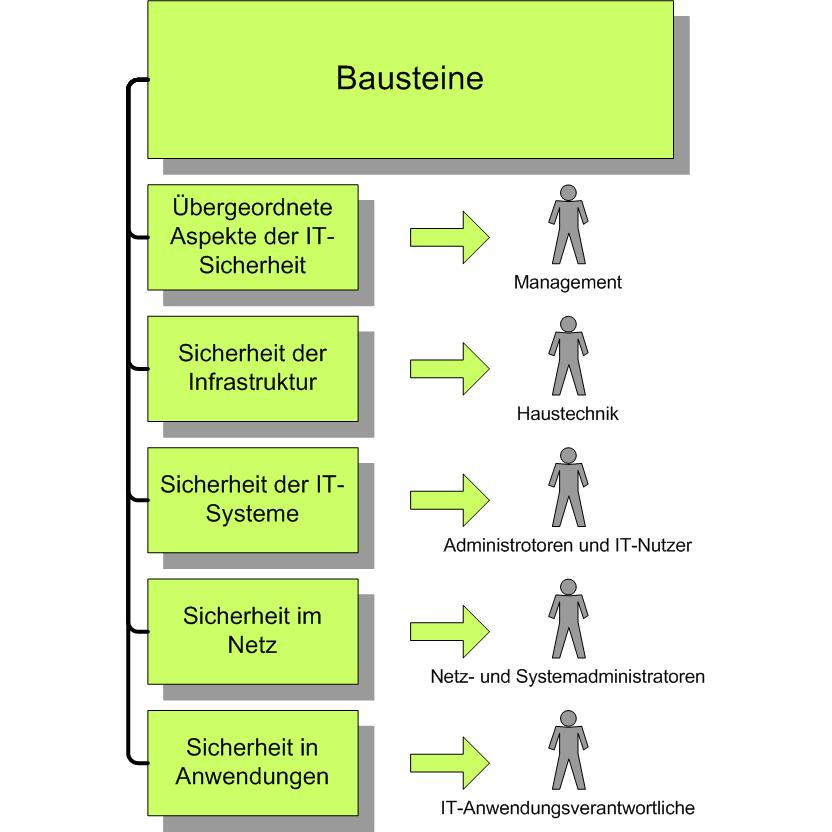
\includegraphics[width=0.8\textwidth,natwidth=832,natheight=832]{figures/Bausteinzuordnung_BSI_Grundschutzkataloge.jpg}
  		}
		}\caption[Firewall:Network]{\DIFaddFL{Firewall-Network}}
		\label{Firewall_Network}
		\todo[inline]{Quelle Wikipedia hinzufügen}
	\end{figure}
	\pagebreak
	\DIFaddend 

	\DIFaddbegin \begin{figure}[htbp]
		\centering
		\DIFaddFL{\fbox{
    		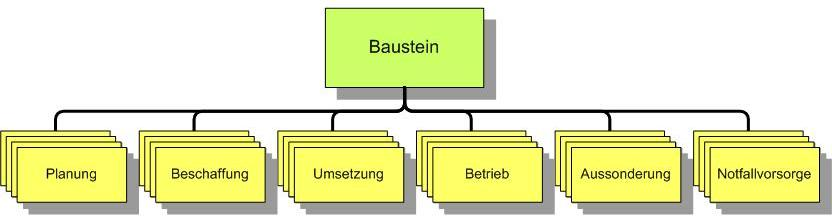
\includegraphics[width=0.8\textwidth,natwidth=832,natheight=218]{figures/Lebenszyklus_BSI_Grundschutzkataloge.jpg}
  		}
		}\caption[Firewall:Network]{\DIFaddFL{Firewall-Network}}
		\label{Firewall_Network}
		\todo[inline]{Quelle Wikipedia hinzufügen}
	\end{figure}

 	\DIFaddend Des Weiteren finden sich Bausteine in Gefährdungskatalogen, welche verschiedene Gefährdungsszenarien 
 	beschreiben und wie folgst lauten:

 	\begin{itemize}
 		\item G 1: Höhere Gewalt
 		\item G 2: Organisatorische Mängel
 		\item G 3: Menschliches Fehlverhalten
 		\item G 4: Technisches Versagen
 		\item G 5: Vorsätzliche Handlungen
 	\end{itemize}
 	\DIFaddbegin \DIFadd{Die Gefährdungskataloge gehen näher auf die möglichen Gefährdungen für IT-Systeme ein.
 	Diese Gefährdungskataloge folgen dem allgemeinen Aufbau nach Schichten.
 	Zur Erstellung des Grundschutzes ist nach Aussagen des BSI das in diesen Katalogen 
 	zusammengestellte Wissen nicht unbedingt notwendig, es fördert jedoch das Verständnis 
 	für die Maßnahme sowie die Wachsamkeit der Verantwortlichen. Die einzelne Gefahrenquelle 
 	ist in einem kurzen Text beschrieben und anschließend werden Beispiele für Schadensfälle, 
 	die durch diese Gefahrenquelle auslösen kann, gegeben.
 	}\DIFaddend \todo[inline]{Quelle hinzufügen}
 	\DIFaddbegin \todo[inline]{Quelle=Wikipedia hinzufügen}
 	\DIFaddend 

 	Welche Maßnahmen und Normen einzuhalten sich um das Sicherheitslevel zu erhöhen, beschreiben die 
 	nachfolgenden sechs Punkte \DIFdelbegin \DIFdel{im }\DIFdelend \DIFaddbegin \DIFadd{in }\DIFaddend Maß\DIFdelbegin \DIFdel{nahmenkatalog}\DIFdelend \DIFaddbegin \DIFadd{nahmenkatalogen}\DIFaddend : 
 	\begin{itemize}
 		\item M 1: Infrastruktur
 		\item M 2: Organisation
 		\item M 3: Personal
 		\item M 4: Hardware und Software
 		\item M 5: Kommunikation
 		\item M 6: Notfallvorsorge
 	\end{itemize}
 	\DIFaddbegin \DIFadd{Die zur Umsetzung des Grundschutzes notwendigen Maßnahmen sind in 
 	Maßnahmenkatalogen zusammengefasst. So werden Maßnahmen, 
 	die für mehrere System-Komponenten angemessen sind, nur einmal zentral beschrieben.
 	Hierbei werden auch Schichten zur Strukturierung der einzelnen Maßnahmengruppen genutzt.
 	In der jeweiligen Maßnahmenbeschreibung sind zunächst Verantwortliche für die Initiierung und 
 	die Umsetzung der Maßnahme genannt. Es folgt eine ausführliche Beschreibung der Maßnahme. 
 	Abschließend werden Kontrollfragen zur korrekten Umsetzung genannt.
 	Bei der Umsetzung der Maßnahmen sollte zunächst überprüft werden, 
 	ob eine Anpassung dieser auf den jeweiligen Betrieb notwendig ist. 
 	Eine genaue Dokumentation solcher Anpassungen ist zur späteren Nachvollziehbarkeit sinnvoll. 
 	Am Ende der Maßnahmen gibt es seit der 10. Ergänzungslieferung sogenannte Prüffragen, 
 	die die wesentlichen Aspekte einer Maßnahme nochmal aufgreifen und somit eine Art Checkliste darstellen,
 	ob diese auch umgesetzt sind.
 	}\todo[inline]{Quelle=Wikipedia hinzufügen}
 	\DIFaddend \todo[inline]{Quelle hinzufügen}

 	Weiters gibt der IT-Grundschutzkatalog \todo[inline]{Quelle hinzufügen} wertvolle Hinweise, 
 	um theoretisch und praktisch einen effektiven Sicherheitsprozess zu gewährleisten.
 \DIFdelbegin %DIFDELCMD < \end{section}
%DIFDELCMD < %%%
\DIFdelend %DIF > \end{section}

 \pagebreak
 \label{Firewalls}
 \begin{section}{Firewalls}
	Das BSI hat sicherheitsspezifische Aspekte für Firewalls beschrieben.
	Sicherheitsspezifische Funktionen sind alle Funktionen einer Firewall, 
	die direkt zum Erreichen der Sicherheitsziele beitragen. \\

	Sicherheitsrelevante Funktionen tragen zum sicheren Funktionieren der Firewall 
	bei und leisten häufig nicht nur Dienste für die sicherheitsspezifischen Funktionen, 
	sondern auch für nicht sicherheitsbezogene Funktionen. Für gewöhnlich hängen 
	sicherheitsspezifische Funktionen vom korrekten Betrieb der sicherheitsrelevanten Funktionen ab. 
	Sicherheitsrelevante Funktionen sind alle Bestandteile, die für die Ausführung der 
	sicherheitsspezifischen Funktionen benötigt werden, also z.B. 
	Teile des Betriebssystems wie Netzwerktreiber, Bibliotheksfunktionen o.Ä. 
	Sie müssen also auch gemäß der oben aufgeführten Evaluationsstufen geprüft werden, 
	wobei auch Wechselwirkungen zu berücksichtigen sind! 
	Zur Erreichung einer größtmöglichen Vereinfachung und Standardisierung sollten die 
	sicherheitsrelevanten Funktionen über eine kleine Anzahl von genau definierten Schnittstellen 
	angesprochen werden können.
	Die sicherheitsspezifischen Funktionen einer Firewall lassen sich wie folgt unterteilen:
	\begin{itemize}
		\item Funktionen zum Schutz gegen direkte Angriffe
		\item Funktionen zum Schutz des zu sichernden Netzes gegen Angriffe aus dem unsicheren Netz
	\end{itemize}
	\todo[inline]{Quelle hinzufügen}
	\pagebreak

  \label{Sicherheitsdienste einer Firewall}
  \begin{subsection}{Sicherheitsdienste einer Firewall}
  	Auf dem Firewall-System werden Sicherheitsmechanismen implementiert, die diesen Übergang 
  	sicher und beherrschbar machen. Dazu analysiert das Firewall-System die Kommunikationsdaten, 
  	kontrolliert die Kommunikationsbeziehungen und Kommunikationspartner, 
  	reglementiert die Kommunikation nach einer Sicherheitspolitik, protokolliert sicherheitsrelevante 
  	Ereignisse und alarmiert bei starken Verstößen den Security-Administrator. \\
  	Nachfolgende Grafik zeigt die exemplarische Einbindung einer Firewall in ein Netzwerk und die Platzierung einer Firewall.
  	%DIF < \centering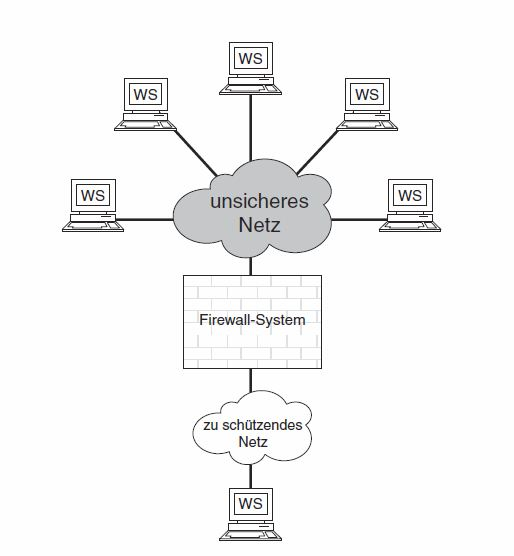
\includegraphics[scale=15%]{figures/Firewall_Nw.jpg}
  	\DIFaddbegin 

  	\DIFaddend \begin{figure}[htbp]
		\centering
		\fbox{\DIFdelbeginFL \DIFdelFL{
    		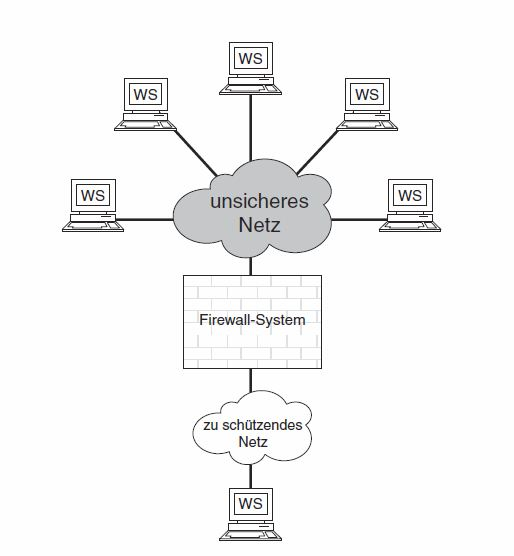
\includegraphics{figures/Firewall_Nw.jpg}
  		}\DIFdelendFL \DIFaddbeginFL \DIFaddFL{
    		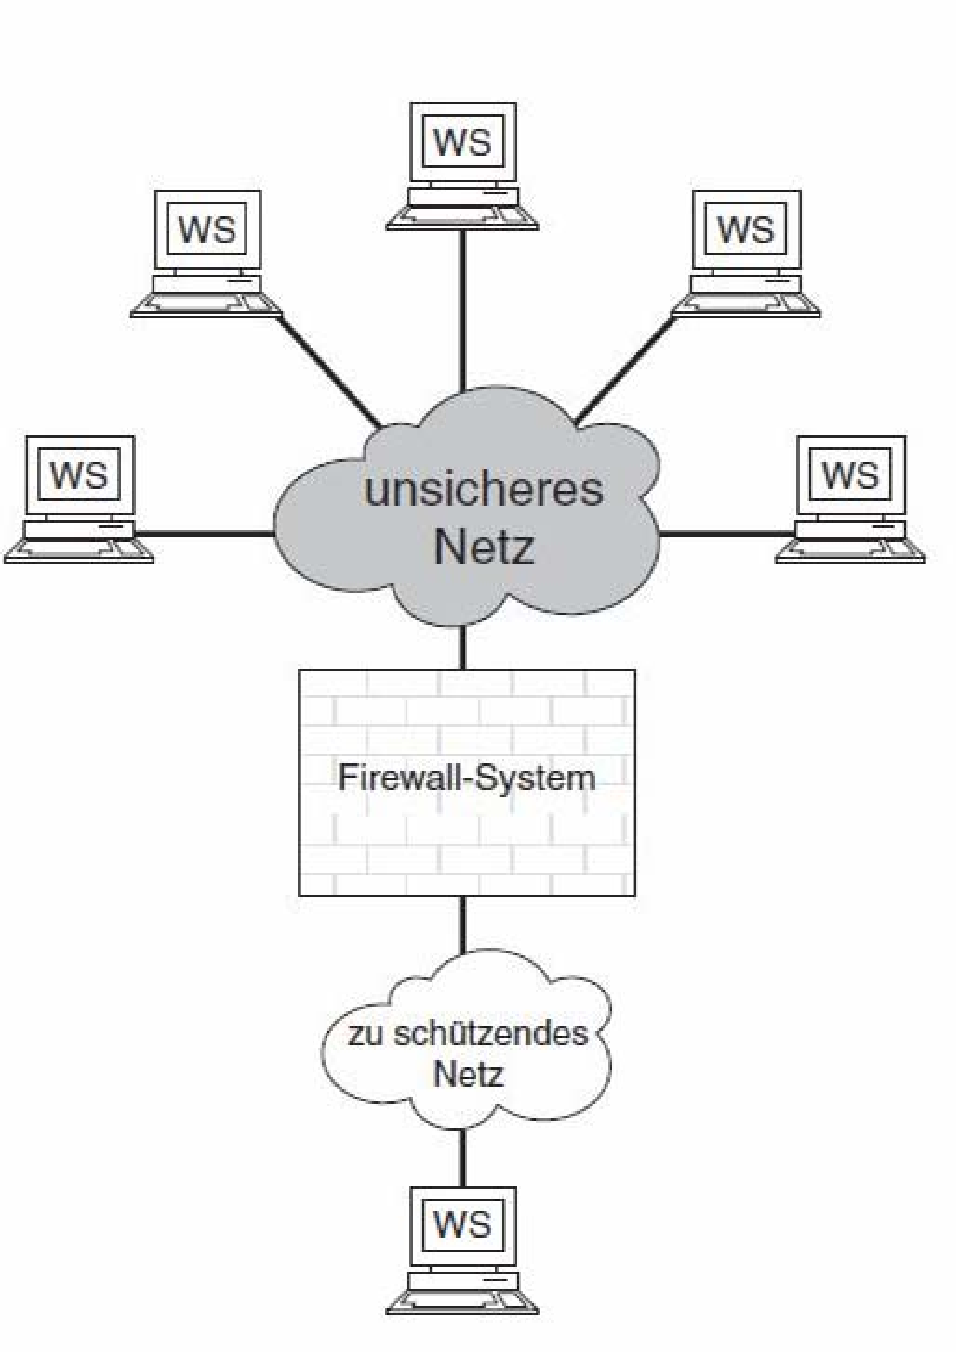
\includegraphics[width=0.8\textwidth,natwidth=514,natheight=556]{figures/Firewall_Nw.pdf}
    		%DIF > [height=60mm, width=100mm]
    		%DIF > \centering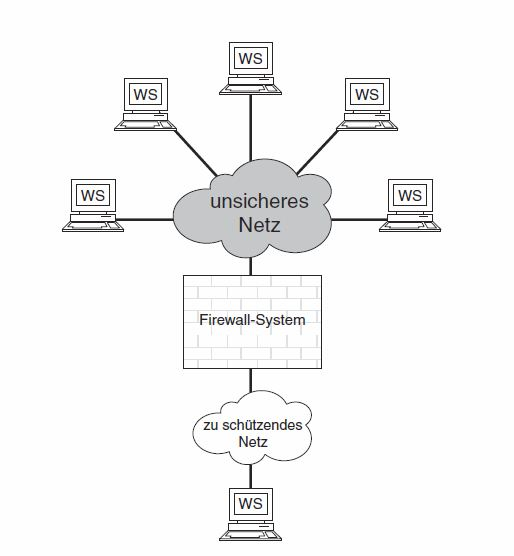
\includegraphics[scale=15%]{figures/Firewall_Nw.jpg}
  		}\DIFaddendFL }
		\caption[Firewall:Network]{Firewall-Network}
		\label{Firewall_Network}
		\todo[inline]{Quelle hinzufügen}
	\end{figure}
  \end{subsection}
  \pagebreak

  \label{Firewall-Konzepte}
  \begin{subsection}{Firewall-Konzepte}
  	Ein Firewall-System stellt den "Common Point of Trust" für den Übergang zwischen 
  	unterschiedlichen Netzen dar, d.h., der einzige Weg ins interne Netz führt kontrolliert über das Firewall-System.
  	\\
  	Firewall-Systeme werden verwendet, um sich an unsichere Netze wie z.B. das Internet anzukoppeln 
  	oder auch, um das eigene Netz zu strukturieren und hier 
  	Sicherheitsdomänen mit unterschiedlichem Schutzbedarf zu schaffen.
  	\todo[inline]{Quelle hinzufügen}

  	\textbf{Vorteile des Common-Point-of-Trust-Konzeptes}
  	\begin{itemize}
  		\item Kosten:
  			Die Realisierung von Sicherheitsmechanismen auf einem zentralen System ist wesentlich einfacher jene 
  			auf jedem einzelnen Rechner.
  		\item Möglichkeiten durch Sicherheitspolitik:
  			Durch eine zentrale Steuerung können die Benutzer einheitlich authentifiziert werden und womöglich 
  			mit kryptographischen Funktionen erweitert werden.
  		\item Abschottung:
  			Durch diese Konzeptionierung kann das zu schützende Netzwerk von unsicheren Netzwerken getrennt werden.
  			Firewall-Systeme können Angriffen entgegenwirken.
  	\end{itemize}
  	\todo[inline]{Quelle hinzufügen}

  	\textbf{Allgemeine Ziele von Firewall-Systemen}
  	\begin{itemize}
  		\item Zugangskontrolle:
  			Auf Daten-, Benutzer- und Netzwerkebene kann die Sicherheit überprüft und gewährleistet werden, 
  			damit ein sicherer Datenaustausch möglich ist.
  		\item Rechteverwaltung:
  			Mittels Protokollen und Diensten kannst festgelegt werden, wann für wen eine Kommunikation über das 
  			Firewall-System erlaubt ist.
  		\item Vertraulichkeit:
  			Die interne Struktur wird hinter dem Schutzsystem verborgen und Nachrichten werden nie im Klartext 
  			übermittelt.
  	\end{itemize}
  	\todo[inline]{Quelle hinzufügen}
  \end{subsection}
 \end{section}
\pagebreak
